\documentclass[aspectratio=169, lualatex, handout]{beamer}
\makeatletter\def\input@path{{theme/}}\makeatother\usetheme{cipher}

\title{Applied Cryptography}
\author{Nadim Kobeissi}
\institute{American University of Beirut}
\instituteimage{images/aub_white.png}
\date{\today}
\coversubtitle{CMPS 297AD/396AI\\Fall 2025}
\coverpartname{Part 2: Real-World Cryptography}
\covertopicname{2.2: The Story of RC4}
\coverwebsite{https://appliedcryptography.page}

\begin{document}
\begin{frame}[plain]
	\titlepage
\end{frame}

\section{About RC4}

\begin{frame}{The Rise and Fall of RC4}
	\begin{itemize}[<+->]
		\item A cryptographic tale of triumph and tragedy
		      \begin{itemize}[<+->]
			      \item \textbf{Birth (1987):} Proprietary stream cipher at RSA Security
			      \item \textbf{Rise (1990s):} Became the world's most widely deployed stream cipher
			      \item \textbf{Golden Era (2000s):} Powered WEP, SSL, and TLS protocols globally
			      \item \textbf{Decline (2001-2015):} A series of devastating cryptanalytic breakthroughs
			      \item \textbf{Demise (2015):} Formal prohibition by IETF, browser vendors
		      \end{itemize}
		\item This story teaches us about cryptographic lifecycle management, the importance of formal security analysis, and the challenges of maintaining backward compatibility
	\end{itemize}
\end{frame}

\begin{frame}{What is RC4?}
	\begin{itemize}[<+->]
		\item \textbf{RC4} (Rivest Cipher 4) is a stream cipher designed for speed and simplicity
		      \begin{itemize}[<+->]
			      \item \textbf{Stream cipher:} Encrypts data one byte at a time
			      \item \textbf{Variable key length:} Supports keys from 1 to 256 bytes
			      \item \textbf{Symmetric encryption:} Same key used for encryption and decryption
		      \end{itemize}
		\item Key characteristics that made it popular:
		      \begin{itemize}[<+->]
			      \item Extremely fast in software (no complex operations)
			      \item Small memory footprint (only 256 bytes of state)
			      \item Simple implementation (just a few lines of code)
		      \end{itemize}
		\item Used extensively in protocols like WEP (Wi-Fi), SSL/TLS, and SSH
	\end{itemize}
\end{frame}

\begin{frame}{Origins of RC4}
	\begin{itemize}[<+->]
		\item \textbf{1987:} Ron Rivest designs RC4 at RSA Security
		      \begin{itemize}[<+->]
			      \item Originally a trade secret, not published
			      \item ``RC'' stands for ``Ron's Code'' or ``Rivest Cipher''
			      \item Designed for practical applications requiring fast encryption
		      \end{itemize}
		\item \textbf{1994:} Algorithm anonymously posted to Cypherpunks mailing list
		      \begin{itemize}[<+->]
			      \item Source code leaked, breaking RSA's trade secret
			      \item Called ``Alleged RC4'' or ``ARCFOUR'' due to legal concerns
			      \item Quickly reverse-engineered and verified as authentic
		      \end{itemize}
		\item \textbf{Impact of the leak:}
		      \begin{itemize}[<+->]
			      \item Made RC4 freely available to implementers worldwide
			      \item Led to its widespread adoption in internet protocols
			      \item Ironically helped RSA by making their cipher ubiquitous
		      \end{itemize}
	\end{itemize}
\end{frame}

\begin{frame}{RC4's Key Scheduling Algorithm (KSA)}
	\begin{itemize}[<+->]
		\item \textbf{Step 1:} Initialize the state array S with values 0 through 255
		      \begin{itemize}[<+->]
			      \item \texttt{for i = 0 to 255: S[i] = i}
		      \end{itemize}
		\item \textbf{Step 2:} Scramble the state array using the key
		      \begin{itemize}[<+->]
			      \item \texttt{j = 0}
			      \item \texttt{for i = 0 to 255:}
			      \item \texttt{\quad j = (j + S[i] + key[i mod keylength]) mod 256}
			      \item \texttt{\quad swap(S[i], S[j])}
		      \end{itemize}
		\item \textbf{Purpose:} Create a pseudo-random permutation of 0-255 based on the key
		\item The quality of this initial scrambling is crucial for security
	\end{itemize}
\end{frame}

\begin{frame}{$\mathsf{PRP}: F_{k}= X \rightarrow X$}{Reminder}
	\begin{columns}[c]
		\begin{column}{0.4\textwidth}
			\begin{itemize}
				\item \textbf{Bijective} (two-way)
				      \begin{itemize}
					      \item \textbf{Injective}: no two inputs map to same output (no
					            collisions)
					      \item \textbf{Surjective}: Every output has one corresponding input
				      \end{itemize}
				\item ``Randomized''
				\item Relations between inputs not reflected in outputs
			\end{itemize}
		\end{column}

		\begin{column}{0.8\textwidth}
			\begin{tikzpicture}[scale=0.38]
				% Define colors
				\definecolor{domaingreen}{RGB}{102, 170, 68}
				\definecolor{rangegreen}{RGB}{102, 170, 68}
				\definecolor{circlecolor}{RGB}{235, 137, 85}
				\definecolor{purplearrow}{RGB}{160, 78, 160}

				% Input space (domain) X - made square
				\draw[dashed, thick, domaingreen, fill=domaingreen]
				(0,0) rectangle (8,8);
				\node[text width=6.5cm, align=center, font=\normalsize]
				at
				(4,-0.8)
				{Size: fixed};
				\node[font=\normalsize] at (4,9) {Input space (domain) $X$};

				% Output (range) Y - made square, same size as domain, moved left
				\draw[thick, rangegreen, fill=rangegreen] (12,0) rectangle (20,8);
				\node[text width=6.5cm, align=center, font=\normalsize]
				at
				(16,-0.8)
				{Size: fixed};
				\node[font=\normalsize] at (16,9) {Output (range) $X$};
				% Input dots - adjusted positions for square domain
				\filldraw[circlecolor] (2,7) circle (0.3);
				\pause
				\draw[-{Stealth[length=6mm, width=4mm]}, thick, purplearrow]
				(2,7) -- (14.2,7.4);
				\pause
				\filldraw[circlecolor] (14.2,7.4) circle (0.3);
				\pause

				\filldraw[circlecolor] (3,6) circle (0.3);
				\pause
				\draw[-{Stealth[length=6mm, width=4mm]}, thick, purplearrow]
				(3,6) -- (18.6,5.3);
				\pause
				\filldraw[circlecolor] (18.6,5.3) circle (0.3);
				\pause

				\filldraw[circlecolor] (2,5) circle (0.3);
				\pause
				\draw[-{Stealth[length=6mm, width=4mm]}, thick, purplearrow]
				(2,5) -- (13.8,4.2);
				\pause
				\filldraw[circlecolor] (13.8,4.2) circle (0.3);
				\pause

				\filldraw[circlecolor] (4,3.5) circle (0.3);
				\pause
				\draw[-{Stealth[length=6mm, width=4mm]}, thick, purplearrow]
				(4,3.5) -- (17.4,2.2);
				\pause
				\filldraw[circlecolor] (17.4,2.2) circle (0.3);
				\pause

				\filldraw[circlecolor] (2,2) circle (0.3);
				\pause
				\draw[-{Stealth[length=6mm, width=4mm]}, thick, purplearrow]
				(2,2) -- (16.1,6.7);
				\pause
				\filldraw[circlecolor] (16.1,6.7) circle (0.3);
				\pause

				\filldraw[circlecolor] (3,1) circle (0.3);
				\pause
				\draw[-{Stealth[length=6mm, width=4mm]}, thick, purplearrow]
				(3,1) -- (19.0,1.4);
				\pause
				\filldraw[circlecolor] (19.0,1.4) circle (0.3);
			\end{tikzpicture}
		\end{column}
	\end{columns}
\end{frame}

\begin{frame}{Limitations of One-Time Pad}{Reminder}
	\definitionbox{The Key Length Problem}{
		One-time pad is not a particularly useful encryption scheme in practice.
	}
	\begin{itemize}[<+->]
		\item The key must be as long as the plaintext!
		\item This creates a chicken-and-egg situation:
		      \begin{itemize}[<+->]
			      \item To privately send $n$ bits of information,
			      \item We must already privately share $n$ bits of information.
		      \end{itemize}
		\item Impractical for most real-world applications.
		      \begin{itemize}[<+->]
			      \item Clearly this is not what we're doing when we use HTTPS,
			      \item or WhatsApp, or pay for something via a debit card...
		      \end{itemize}
		\item We need encryption schemes where the key can be smaller than the message.
	\end{itemize}
\end{frame}

\begin{frame}{Idea: find a way to expand the key}{Reminder}
	\begin{itemize}[<+->]
		\item Given a key $k_s$ of size $\left|k_s\right| < \left|m\right|$, find a way to obtain $\left|k_e\right| \geq \left|m\right|$
		\item In the real world, we have two kinds of symmetric encryption schemes:
		      \begin{itemize}[<+->]
			      \item \textbf{Block ciphers}: AES, 3DES, etc.
			      \item \textbf{Stream ciphers}: ChaCha20, RC4, etc.
		      \end{itemize}
		\item This is exactly what stream ciphers do!
		      \begin{itemize}[<+->]
			      \item Start with a small key $k_s$ of a fixed size $\left|k_s\right| = \lambda$,
			      \item Magically expand it to $k_e$ where $\left|k_e\right| \geq \left|m\right|$,
			      \item $\func{enc}{K, M} = K \oplus M$
		      \end{itemize}
	\end{itemize}
\end{frame}

\begin{frame}{RC4's Pseudo-Random Generation Algorithm (PRGA)}
	\begin{itemize}[<+->]
		\item \textbf{Initialization:} Set counters \texttt{i = 0, j = 0}
		\item \textbf{For each byte to encrypt:}
		      \begin{itemize}[<+->]
			      \item \texttt{i = (i + 1) mod 256}
			      \item \texttt{j = (j + S[i]) mod 256}
			      \item \texttt{swap(S[i], S[j])}
			      \item \texttt{K = S[(S[i] + S[j]) mod 256]} \quad ← keystream byte
			      \item \texttt{ciphertext = plaintext XOR K}
		      \end{itemize}
		\item \textbf{Key insight:} The state array S is continuously modified
		      \begin{itemize}[<+->]
			      \item Each keystream byte depends on the entire previous history
			      \item Creates a very long period before repetition
		      \end{itemize}
		\item \textbf{Decryption:} Identical process (XOR is self-inverse)
	\end{itemize}
\end{frame}

\begin{frame}{RC4's golden age (1990s-2000s)}
	\begin{itemize}[<+->]
		\item \textbf{The most widely deployed stream cipher in history}
		      \begin{itemize}[<+->]
			      \item Estimated to secure over 50\% of all SSL/TLS connections at its peak
			      \item Billions of devices worldwide relied on RC4 for encryption
		      \end{itemize}
		\item \textbf{Ubiquitous protocol adoption:}
		      \begin{itemize}[<+->]
			      \item \textbf{WEP (1997):} Wi-Fi security standard used RC4 exclusively
			      \item \textbf{SSL 3.0/TLS 1.0 (1995-1999):} RC4 as preferred cipher suite
			      \item \textbf{SSH-1 (1995):} Early secure shell implementations
			      \item \textbf{Microsoft Office:} Document password protection
			      \item \textbf{Adobe PDF:} File encryption standard
		      \end{itemize}
		\item \textbf{Why RC4 dominated:}
		      \begin{itemize}[<+->]
			      \item 5-10x faster than DES in software implementations
			      \item Minimal memory requirements (perfect for embedded systems)
			      \item No export restrictions (unlike strong block ciphers)
			      \item Simple to implement correctly
		      \end{itemize}
	\end{itemize}
\end{frame}

\section{RSA in WEP}

\begin{frame}{Early RC4 weaknesses (1995-2000)}
	\begin{itemize}[<+->]
		\item \textbf{1995:} First statistical biases discovered by Wagner and Goldberg
		      \begin{itemize}[<+->]
			      \item Found that the second byte of RC4 keystream was biased
			      \item Probability of being zero was $2/256$ instead of $1/256$
			      \item Seemed like a minor curiosity at the time...
		      \end{itemize}
		\item \textbf{1997:} Golic discovered more biases in the keystream
		      \begin{itemize}[<+->]
			      \item Certain byte positions showed statistical irregularities
			      \item Still considered mostly theoretical concerns
		      \end{itemize}
		\item \textbf{2000:} Jenkins found patterns in RC4's internal state
		      \begin{itemize}[<+->]
			      \item Identified correlations between consecutive keystream bytes
			      \item Cryptographic community began to worry about RC4's security
		      \end{itemize}
		\item \textbf{The stage was set} for a more devastating attack...
	\end{itemize}
\end{frame}

\begin{frame}{Weak keys in KSA}
	\begin{columns}[c]
		\begin{column}{1\textwidth}
			\begin{itemize}[<+->]
				\item \textbf{The Discovery:} Certain key patterns create predictable initial states\footnote{\url{https://appliedcryptography.page/papers/\#rc4-ksa}}
				\item \textbf{Weak Key Pattern:} Keys of the form $(K_1, K_2, \ldots, K_n, 3, 255, \ldots)$
				      \begin{itemize}[<+->]
					      \item When byte 3 of the key is 3, and byte 4 is 255
					      \item The KSA creates a predictable correlation in the state array
				      \end{itemize}
				\item \textbf{The Mathematics:}
				      \begin{itemize}[<+->]
					      \item After KSA completes, $S[1] = 3$ with high probability
					      \item In the first step of PRGA: $i = 1, j = S[1] = 3$
					      \item First keystream byte: $S[S[1] + S[3]] = S[3 + S[3]]$
					      \item This reveals information about the key!
				      \end{itemize}
				\item \textbf{Frequency:} About 1 in 256 keys exhibit this weakness
			\end{itemize}
		\end{column}
	\end{columns}
\end{frame}

\begin{frame}{One-time secrecy of a SKE}{Reminder}
	\begin{columns}[c]
		\begin{column}{0.5\textwidth}
			\definitionbox{One-time Secrecy for SKE}{
				An SKE scheme $\Sigma$ has one-time secrecy if the following libraries are interchangeable:
				\vspace{0.5mm}
				\begin{center}
					\sslinked{
						\sslibrary{\Sigma}{ots-real}{
							\sslibrarysubroutine{ots.enc}{M}{
								$K \twoheadleftarrow \Sigma.\mathcal{K}$ \\
								$C \coloneq \Sigma.\textsf{Enc}(K, M)$ \\
								return $C$
							}{1}
						}{0.8}
					}{\interchangeable{}}{
						\sslibrary{\Sigma}{ots-rand}{
							\sslibrarysubroutine{ots.enc}{M}{
								$C \twoheadleftarrow \Sigma.\mathcal{C}$ \\
								return $C$
							}{1}
						}{0.8}
					}
				\end{center}
			}
		\end{column}
		\begin{column}{0.5\textwidth}
			An encryption scheme has one-time secrecy if its ciphertexts are uniformly distributed, when keys are sampled uniformly, kept secret, and used for only one encryption, and no matter how the plaintexts are chosen.
			\\
			\textbf{Does this apply to RC4, especially after the attacks?}
		\end{column}
	\end{columns}
\end{frame}

\begin{frame}{Attacks mean distinguishability}{RC4 getting less and less ``indistinguishable from random''}
	\begin{columns}[c]
		\begin{column}{0.35\textwidth}
			\sssubroutine{RC4Encrypt}{M}{
				$k \twoheadleftarrow \bits^{\lambda}$ \\
				$K \coloneq \texttt{RC4}(k, |M|)$ \\
				$C \coloneq K \oplus M$ \\
				return $C$
			}{1.5}
		\end{column}
		\begin{column}{0.3\textwidth}
			\begin{center}
				{\huge{$\cancel{\approxeq}$}} \\[1em]
			\end{center}
		\end{column}
		\begin{column}{0.35\textwidth}
			\sssubroutine{Random}{M}{
				$C \twoheadleftarrow \bits^{|M|}$ \\
				return $C$
			}{1.5}
		\end{column}
	\end{columns}
\end{frame}

\begin{frame}{In fact...}
	\bigimagewithcaption{rc4_bias.png}{Source: Kenny Paterson}
\end{frame}

\begin{frame}{Attacks: from theory to practice}
	\begin{itemize}[<+->]
		\item \textbf{Step 1:} Collect many ciphertexts encrypted with related keys
		      \begin{itemize}[<+->]
			      \item Keys that differ only in the first few bytes
			      \item Wait for keys with the vulnerable pattern to appear
		      \end{itemize}
		\item \textbf{Step 2:} Identify weak keys from keystream patterns
		      \begin{itemize}[<+->]
			      \item Look for the telltale signatures in the first keystream byte
			      \item Discard non-vulnerable encryptions
		      \end{itemize}
		\item \textbf{Step 3:} Recover key bytes incrementally
		      \begin{itemize}[<+->]
			      \item Use the correlation to determine likely values for key bytes
			      \item Build up the key one byte at a time
		      \end{itemize}
		\item \textbf{Success rate:} With enough samples, key recovery becomes highly reliable
	\end{itemize}
\end{frame}

\begin{frame}{How WEP encryption works}
	\begin{columns}[c]
		\begin{column}{0.5\textwidth}
			\begin{itemize}[<+->]
				\item \textbf{Components:}
				      \begin{itemize}[<+->]
					      \item 24-bit IV (Initialization Vector)
					      \item 104-bit PSK (pre-shared key)
					            \begin{itemize}
						            \item Derived from Wi-Fi password
						            \item Was limited to 40 bits at first due to US export controls!
					            \end{itemize}
				      \end{itemize}
				\item \textbf{Process:}
				      \begin{itemize}[<+->]
					      \item Choose random IV for each packet
					      \item Concatenate: IV $\|$ Secret Key
					      \item Feed to RC4 to generate keystream
					      \item XOR plaintext with keystream
				      \end{itemize}
			\end{itemize}
			\begin{center}
				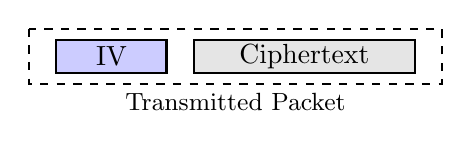
\begin{tikzpicture}[scale=0.7]
					% Transmitted packet
					\draw[thick, dashed] (-0.5,-5) rectangle (7,-6);
					\draw[thick, fill=blue!20] (0,-5.2) rectangle (2,-5.8);
					\node at (1,-5.5) {IV};
					\draw[thick, fill=gray!20] (2.5,-5.2) rectangle (6.5,-5.8);
					\node at (4.5,-5.5) {Ciphertext};
					\node[below] at (3.25,-6) {\small Transmitted Packet};
				\end{tikzpicture}
			\end{center}
		\end{column}
		\begin{column}{0.5\textwidth}
			\begin{center}
				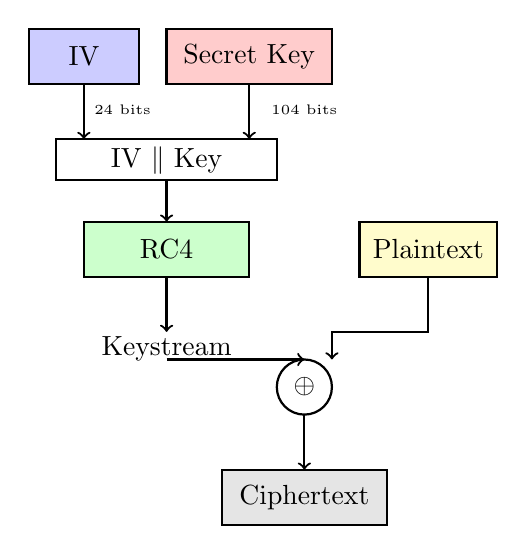
\begin{tikzpicture}[scale=0.7]
					% IV Box
					\draw[thick, fill=blue!20] (0,4) rectangle (2,5);
					\node at (1,4.5) {IV};
					\node[below] at (1.7,3.8) {\tiny 24 bits};

					% Secret Key Box
					\draw[thick, fill=red!20] (2.5,4) rectangle (5.5,5);
					\node at (4,4.5) {Secret Key};
					\node[below] at (5,3.8) {\tiny 104 bits};

					% Concatenation
					\draw[->, thick] (1,4) -- (1,3);
					\draw[->, thick] (4,4) -- (4,3);
					\draw[thick] (0.5,2.25) rectangle (4.5,3);
					\node at (2.5,2.6) {IV $\|$ Key};

					% RC4 Box
					\draw[->, thick] (2.5,2.25) -- (2.5,1.5);
					\draw[thick, fill=green!20] (1,0.5) rectangle (4,1.5);
					\node at (2.5,1) {RC4};

					% Keystream
					\draw[->, thick] (2.5,0.5) -- (2.5,-0.5);
					\node at (2.5,-0.8) {Keystream};

					% Plaintext
					\draw[thick, fill=yellow!20] (6,0.5) rectangle (8.5,1.5);
					\node at (7.25,1) {Plaintext};

					% XOR
					\draw[->, thick] (2.5,-1) -- (5,-1);
					\draw[->, thick] (7.25,0.5) -- (7.25,-0.5) -- (5.5,-0.5) -- (5.5,-1);
					\draw[thick] (5,-1.5) circle (0.5);
					\node at (5,-1.5) {$\oplus$};

					% Ciphertext
					\draw[->, thick] (5,-2) -- (5,-3);
					\draw[thick, fill=gray!20] (3.5,-3) rectangle (6.5,-4);
					\node at (5,-3.5) {Ciphertext};
				\end{tikzpicture}
			\end{center}
		\end{column}
	\end{columns}
\end{frame}

\begin{frame}{WEP: the perfect storm}
	\begin{columns}[c]
		\begin{column}{1\textwidth}
			\begin{itemize}[<+->]
				\item \textbf{WEP (Wired Equivalent Privacy):} Wi-Fi security protocol from 1997
				      \begin{itemize}[<+->]
					      \item Used RC4 for encryption
					      \item 104-bit secret key shared among all devices
				      \end{itemize}
				\item \textbf{Vulnerable design choice:} Initialization Vectors (IVs)
				      \begin{itemize}[<+->]
					      \item To avoid key reuse, WEP prepends a 24-bit IV to each packet
					      \item RC4 key becomes: $(IV_1, IV_2, IV_3, K_1, K_2, \ldots, K_n)$
					      \item IV is sent \emph{in plaintext} with each packet!
				      \end{itemize}
				\item \textbf{Break:} This creates exactly the conditions the FMS (Fluhrer, Mantin, Shamir) attack exploited
				      \begin{itemize}[<+->]
					      \item Many related keys (same secret key, different IVs)
					      \item Attacker knows the first 3 bytes of each key (the IV)
					      \item Perfect setup for the FMS attack!
				      \end{itemize}
			\end{itemize}
		\end{column}
	\end{columns}
\end{frame}

\begin{frame}{WEP's IV structure}
	\begin{center}
		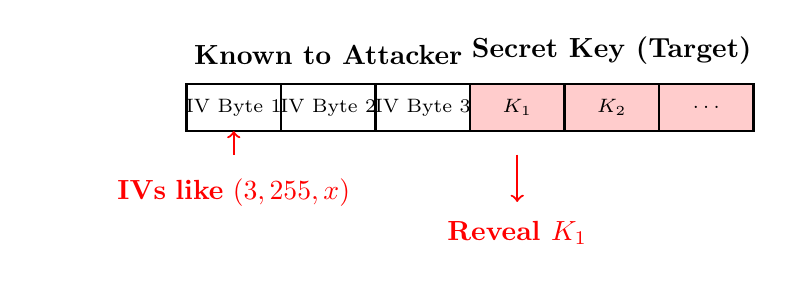
\begin{tikzpicture}[scale=0.6]
			\draw[thick] (0,2) rectangle (2,3);
			\node at (1,2.5) {\scriptsize IV Byte 1};
			\draw[thick] (2,2) rectangle (4,3);
			\node at (3,2.5) {\scriptsize IV Byte 2};
			\draw[thick] (4,2) rectangle (6,3);
			\node at (5,2.5) {\scriptsize IV Byte 3};
			\draw[thick, fill=red!20] (6,2) rectangle (8,3);
			\node at (7,2.5) {\scriptsize $K_1$};
			\draw[thick, fill=red!20] (8,2) rectangle (10,3);
			\node at (9,2.5) {\scriptsize $K_2$};
			\draw[thick, fill=red!20] (10,2) rectangle (12,3);
			\node at (11,2.5) {\scriptsize $\ldots$};
			\node[above] at (3,3.2) {\textbf{Known to Attacker}};
			\node[above] at (9,3.2) {\textbf{Secret Key (Target)}};n
			\draw[->, thick, red] (1,1.5) -- (1,2);
			\node[below, red, text width=5cm, align=center] at (1,1.2) {\textbf{IVs like $(3, 255, x)$}};
			\draw[->, thick, red] (7,1.5) -- (7,0.5);
			\node[below, red] at (7,0.3) {\textbf{Reveal $K_1$}};
		\end{tikzpicture}
	\end{center}
	\begin{itemize}[<+->]
		\item \textbf{The FMS Attack:} Exploits weak IV patterns of form $(A+3, 255, x)$
		\item \textbf{Pattern:} To attack key byte $K_A$, wait for IVs $(A+3, 255, x)$
		\item \textbf{Frequency:} About 1 in 65,536 packets match the vulnerable pattern
		\item \textbf{Collection:} Need multiple matching IVs per key byte for statistical attack
		\item \textbf{Result:} With enough packets, incrementally recover the entire key
	\end{itemize}
\end{frame}

\begin{frame}{Practical tools}
	\begin{itemize}[<+->]
		\item \textbf{AirSnort (2001):} First practical WEP cracking tool
		      \begin{itemize}[<+->]
			      \item Implemented the FMS attack
			      \item Could crack WEP keys with 1-5 million packets
			      \item Made WEP cracking accessible to non-experts
		      \end{itemize}
		\item \textbf{WEPCrack (2001):} Another early implementation
		      \begin{itemize}[<+->]
			      \item Demonstrated the attack's effectiveness
			      \item Confirmed that WEP was fundamentally broken
		      \end{itemize}
		\item \textbf{Aircrack-ng (2006):} Improved and optimized tools
		      \begin{itemize}[<+->]
			      \item Reduced required packets to hundreds of thousands
			      \item Added packet injection to speed up attacks
			      \item Still widely used today for security testing
		      \end{itemize}
	\end{itemize}
\end{frame}

\begin{frame}{Attack: step by step}
	\begin{itemize}[<+->]
		\item \textbf{Step 1:} Attacker sets Wi-Fi card to monitor mode
		      \begin{itemize}[<+->]
			      \item Passively collects all WEP-encrypted packets
			      \item No need to associate with the target network
		      \end{itemize}
		\item \textbf{Step 2:} Filter for packets with vulnerable IVs
		      \begin{itemize}[<+->]
			      \item Look for ``weak IVs''
			      \item Collect the corresponding keystream bytes
		      \end{itemize}
		\item \textbf{Step 3:} Apply statistical analysis
		      \begin{itemize}[<+->]
			      \item Use FMS attack to determine most likely key byte values
			      \item Incrementally build up the secret key
		      \end{itemize}
		\item \textbf{Step 4:} Verify the recovered key
		      \begin{itemize}[<+->]
			      \item Test against captured packets
			      \item Success: Complete compromise of the Wi-Fi network!
		      \end{itemize}
	\end{itemize}
\end{frame}

\begin{frame}{Attacks only get better}
	\begin{itemize}[<+->]
		\item \textbf{Klein's Attack (2005):} Extended the vulnerable IV patterns
		      \begin{itemize}[<+->]
			      \item Found additional weak key structures
			      \item Reduced the number of packets needed for key recovery
		      \end{itemize}
		\item \textbf{PTW Attack (2007):} Pyshkin, Tews, and Weinmann
		      \begin{itemize}[<+->]
			      \item Revolutionary approach using Bayes' theorem
			      \item Could crack WEP with as few as 40,000 packets
			      \item Made attacks feasible on even low-traffic networks
		      \end{itemize}
		\item \textbf{Key Recovery Speedup:} From hours to minutes
		      \begin{itemize}[<+->]
			      \item Modern attacks can crack WEP in under 10 minutes
			      \item Some demonstrations crack it in under 60 seconds
		      \end{itemize}
	\end{itemize}
\end{frame}

\begin{frame}{Lessons learned from WEP}
	\begin{itemize}[<+->]
		\item \textbf{Lesson 1:} Never use a stream cipher with related keys
		      \begin{itemize}[<+->]
			      \item WEP's IV structure created exactly this scenario
			      \item Modern protocols use proper key derivation functions
		      \end{itemize}
		\item \textbf{Lesson 2:} Academic attacks become practical faster than expected
		      \begin{itemize}[<+->]
			      \item FMS attack went from paper to tool in months
			      \item ``Theoretical'' often means ``practical soon''
		      \end{itemize}
		\item \textbf{Lesson 3:} Security protocols need formal analysis
		      \begin{itemize}[<+->]
			      \item WEP was designed by committee without cryptographic rigor
			      \item Modern protocols undergo extensive peer review
		      \end{itemize}
		\item \textbf{Lesson 4:} Backward compatibility can be a security nightmare
		      \begin{itemize}[<+->]
			      \item WEP remained deployed long after being broken
			      \item Organizations were slow to migrate due to cost/complexity
		      \end{itemize}
	\end{itemize}
\end{frame}

\begin{frame}{WEP timeline}
	\begin{itemize}[<+->]
		\item \textbf{2001:} FMS attack published - WEP theoretically broken
		\item \textbf{2001:} AirSnort released - WEP practically broken
		\item \textbf{2003:} WPA (Wi-Fi Protected Access) standardized as replacement
		\item \textbf{2004:} WPA2 released with AES encryption
		\item \textbf{2006:} Wi-Fi Alliance deprecates WEP
		\item \textbf{2012:} WEP support removed from Windows 8
		\item \textbf{2018:} Many vendors stop supporting WEP entirely
		\item \textbf{Today:} WEP is considered a historical curiosity
	\end{itemize}
\end{frame}

\section{RC4 in TLS}

\begin{frame}{RC4 in TLS: from preferred to prohibited}
	\begin{itemize}[<+->]
		\item \textbf{RC4's role in TLS/SSL:} Once the default stream cipher
		      \begin{itemize}[<+->]
			      \item Preferred over block ciphers due to speed
			      \item No need for padding (unlike CBC mode)
			      \item Avoided the BEAST attack against CBC ciphers
		      \end{itemize}
		\item \textbf{2011:} BEAST attack made RC4 more attractive
		      \begin{itemize}[<+->]
			      \item Attack on CBC mode in TLS 1.0
			      \item Many servers switched to RC4-only cipher suites
			      \item RC4 usage actually increased!
		      \end{itemize}
		\item \textbf{The irony:} Avoiding one attack led directly into another
		      \begin{itemize}[<+->]
			      \item RC4's biases were known but considered impractical
			      \item This assumption would prove catastrophically wrong
		      \end{itemize}
	\end{itemize}
\end{frame}

\begin{frame}{AlFardan et al. (2013): RC4 biases in TLS}
	\begin{columns}[c]
		\begin{column}{0.6\textwidth}
			\begin{itemize}[<+->]
				\item \textbf{The discovery:} RC4's biases are exploitable in TLS:\footnote{\url{https://appliedcryptography.page/papers/\#rc4-tls}}
				      \begin{itemize}[<+->]
					      \item First 256 bytes of keystream heavily biased
					      \item Certain byte positions more predictable than others
					      \item Biases persist even with proper key generation
				      \end{itemize}
				\item \textbf{Key finding:} Single-byte biases
				      \begin{itemize}[<+->]
					      \item Position 1: $\Pr[Z_1 = 0] \approx 2^{-7}$ (double expected)
					      \item Position 2: $\Pr[Z_2 = 0] \approx 2^{-7}$ (double expected)
					      \item Positions 3-255: Various smaller biases
				      \end{itemize}
			\end{itemize}
		\end{column}
		\begin{column}{0.4\textwidth}
			\begin{itemize}[<+->]
				\item \textbf{Multi-byte biases:} Even stronger patterns
				      \begin{itemize}[<+->]
					      \item $(Z_1, Z_{257}) = (0, 0)$ with probability $2^{-11}$
					      \item Should be $2^{-16}$ if truly random
					      \item 32 times more likely than expected!
				      \end{itemize}
			\end{itemize}
		\end{column}
	\end{columns}
\end{frame}

\begin{frame}{The broadcast attack scenario}
	\begin{itemize}[<+->]
		\item \textbf{Attack model:} Same plaintext encrypted many times
		      \begin{itemize}[<+->]
			      \item HTTP cookies sent with every request
			      \item Session tokens in fixed positions
			      \item Password fields in web forms
		      \end{itemize}
		\item \textbf{The mathematics:} Bias accumulation
		      \begin{itemize}[<+->]
			      \item Collect ciphertexts: $C_1, C_2, \ldots, C_n$
			      \item For position $i$: count occurrences of each byte value
			      \item Most frequent ciphertext byte reveals plaintext byte
			      \item Required samples: $\mathcal{O}(N \cdot B^{-2})$ where $B$ is bias
		      \end{itemize}
		\item \textbf{Practical requirements:}
		      \begin{itemize}[<+->]
			      \item $2^{24}$ to $2^{30}$ encryptions needed
			      \item Feasible for persistent attackers
			      \item JavaScript injection can generate traffic
		      \end{itemize}
	\end{itemize}
\end{frame}

\begin{frame}{Garman et al. (2015): attacks only get better}
	\begin{columns}[c]
		\begin{column}{0.5\textwidth}
			\begin{itemize}[<+->]
				\item \textbf{The challenge:} AlFardan et al.'s attack was still ``impractical''
				      \begin{itemize}[<+->]
					      \item Required billions of encryptions
					      \item Took days or weeks to execute
					      \item Many dismissed it as theoretical
				      \end{itemize}
				\item \textbf{Insight:} Target password verifiers, not cookies\footnote{\url{https://appliedcryptography.page/papers/\#rc4-attacks}}
				      \begin{itemize}[<+->]
					      \item Basic Authentication sends passwords in every request
					      \item IMAP/SMTP use similar repeated authentication
					      \item Password structure provides additional constraints
				      \end{itemize}
			\end{itemize}
		\end{column}
		\begin{column}{0.5\textwidth}
			\begin{itemize}[<+->]
				\item \textbf{The improvements:} Orders of magnitude faster
				      \begin{itemize}[<+->]
					      \item Exploit password character distributions
					      \item Use Mantin's ABSAB bias (positions 1-4)
					      \item Combine with dictionary attacks
					      \item Other attack papers use similar techniques, including to break WPA-TKIP, a successor to WEP!\footnote{\url{https://appliedcryptography.page/papers/\#rc4-biases}}
				      \end{itemize}
			\end{itemize}
		\end{column}
	\end{columns}
\end{frame}

\begin{frame}{Mantin's ABSAB bias (2005)}
	\begin{itemize}[<+->]
		\item \textbf{The discovery:} Certain digraph patterns repeat with anomalous frequency\footnote{\url{https://appliedcryptography.page/papers/\#rc4-absab}}
		      \begin{itemize}[<+->]
			      \item Pattern: Two characters repeat after a gap (e.g., ABAB, ABCAB)
			      \item Occurs when value 1 is used to update index $j$ in RC4
			      \item Creates correlations between distant output positions
		      \end{itemize}
		\item \textbf{The mathematics:} For pattern AB...AB with gap $G$
		      \begin{itemize}[<+->]
			      \item Expected probability in random: $1/N^2$
			      \item Actual probability in RC4: $(1 + e^{(-4-8G)/N}/N) \cdot 1/N^2$
			      \item Relative bias: $\approx 1/N$ for zero gap, decreases with gap size
		      \end{itemize}
		\item \textbf{Why it matters:}
		      \begin{itemize}[<+->]
			      \item Enables distinguishing attacks with only $2^{26}$ samples
			      \item Can predict individual bytes with 82\% accuracy after $2^{50}$ samples
			      \item Particularly effective against password-based authentication
		      \end{itemize}
	\end{itemize}
\end{frame}

\begin{frame}{ABSAB bias in action: practical example}
	\begin{itemize}[<+->]
		\item \textbf{Target:} Password ``hello123'' in HTTP Basic Authentication
		\item \textbf{Step 1:} Password encoded as base64: ``aGVsbG8xMjM=''
		\item \textbf{Step 2:} Look for ABSAB patterns in collected ciphertexts:
		      \begin{center}
			      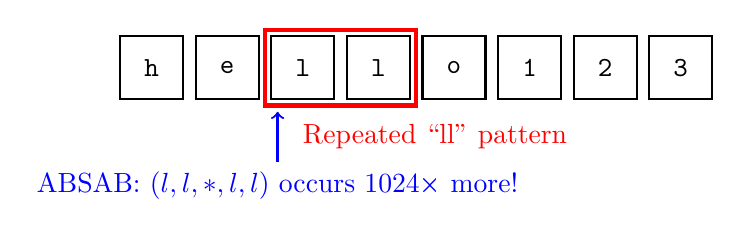
\begin{tikzpicture}[scale=0.8]
				      \foreach \i/\char in {0/h,1/e,2/l,3/l,4/o,5/1,6/2,7/3} {
						      \draw[thick] (\i*1.2,2) rectangle (\i*1.2+1,3);
						      \node at (\i*1.2+0.5,2.5) {\texttt{\char}};
					      }
				      \draw[red, ultra thick] (2*1.2-0.1,1.9) rectangle (3*1.2+1.1,3.1);
				      \node[red, below] at (5,1.75) {Repeated ``ll'' pattern};
				      \draw[->, thick, blue] (2.5,1) -- (2.5,1.8);
				      \node[blue, below] at (2.5,1) {ABSAB: $(l,l,*,l,l)$ occurs 1024× more!};
			      \end{tikzpicture}
		      \end{center}
		\item \textbf{Step 3:} After $2^{26}$ samples, frequency analysis reveals:
		      \begin{itemize}[<+->]
			      \item Positions 2-3: ``ll'' pattern confirmed via ABSAB
			      \item Position 0: ``h'' (68/256 occurrences)
			      \item Position 1: ``e'' (65/256 occurrences)
			      \item Password structure revealed: ``h\_ll\_\_\_\_''
		      \end{itemize}
		\item \textbf{Result:} Search space reduced from $62^8$ to $62^4$ possibilities!
	\end{itemize}
\end{frame}

\begin{frame}{Password recovery: the numbers}
	\begin{itemize}[<+->]
		\item \textbf{Basic Authentication attack performance:}
		      \begin{itemize}[<+->]
			      \item 6-character passwords: $2^{26}$ encryptions
			      \item Time: ~50-100 hours.
		      \end{itemize}
		\item \textbf{IMAP attack results:}
		      \begin{itemize}[<+->]
			      \item Real passwords recovered in laboratory setting
			      \item Character-by-character recovery possible
		      \end{itemize}
	\end{itemize}
\end{frame}

\begin{frame}{POODLE (2014): the final nail}
	\begin{itemize}[<+->]
		\item \textbf{POODLE:} Padding Oracle On Downgraded Legacy Encryption
		      \begin{itemize}[<+->]
			      \item Not specifically an RC4 attack
			      \item But exploited SSL 3.0's MAC-then-encrypt with CBC
			      \item Led to mass exodus from SSL 3.0
		      \end{itemize}
		\item \textbf{The downgrade dance:}
		      \begin{itemize}[<+->]
			      \item Attackers force TLS connections to fail
			      \item Browsers retry with older SSL 3.0
			      \item SSL 3.0 has no downgrade protection!
		      \end{itemize}
		\item \textbf{Why this matters for RC4:}
		      \begin{itemize}[<+->]
			      \item SSL 3.0 heavily used RC4
			      \item POODLE + RC4 biases = from compromise to compromise
			      \item Final push to deprecate both SSL 3.0 and RC4
		      \end{itemize}
	\end{itemize}
\end{frame}

\begin{frame}{Coordinated response between vendors}
	\begin{itemize}[<+->]
		\item \textbf{2013:} IETF begins discussing RC4 deprecation
		      \begin{itemize}[<+->]
			      \item Working groups start planning migration
		      \end{itemize}
		\item \textbf{2014/2015:} Major browsers act
		      \begin{itemize}[<+->]
			      \item Chrome/Firefox announce RC4 phase-out plans
			      \item Microsoft issues security advisories
			      \item Apple begins removing RC4 from Safari
		      \end{itemize}
		\item \textbf{2015:} RFC 7465 prohibits RC4 in TLS
		      \begin{itemize}[<+->]
			      \item ``TLS clients MUST NOT include RC4 cipher suites''
			      \item ``TLS servers MUST NOT select RC4 cipher suites''
			      \item Formal end of RC4 in internet protocols
		      \end{itemize}
		\item \textbf{2016/2018:} RC4 removed from all major browsers
	\end{itemize}
\end{frame}

\begin{frame}{Technical lessons from RC4's demise}
	\begin{itemize}[<+->]
		\item \textbf{Lesson 1:} Statistical biases matter at scale
		      \begin{itemize}[<+->]
			      \item ``Small'' biases become exploitable with enough data
			      \item Modern internet generates massive data volumes
			      \item Never dismiss statistical irregularities
		      \end{itemize}
		\item \textbf{Lesson 2:} Attacks combine in unexpected ways
		      \begin{itemize}[<+->]
			      \item ABSAB bias + password structure = practical attack
			      \item Protocol downgrade + cipher weakness = disaster
		      \end{itemize}
		\item \textbf{Lesson 3:} Migration is painful but necessary
		      \begin{itemize}[<+->]
			      \item RC4 removal broke many legacy systems
			      \item But waiting would have been catastrophic
			      \item Plan for crypto-agility from the start
		      \end{itemize}
	\end{itemize}
\end{frame}

\begin{frame}{RC4: a complete timeline}
	\begin{itemize}[<+->]
		\item \textbf{1987:} Ron Rivest designs RC4
		\item \textbf{1994:} Algorithm leaked to cypherpunks
		\item \textbf{1995-2000:} Early bias discoveries
		\item \textbf{2001:} FMS attack breaks WEP
		\item \textbf{2011:} BEAST attack increases RC4 usage
		\item \textbf{2013:} AlFardan et al. show TLS attacks are almost practical
		\item \textbf{2014:} POODLE compromises SSL 3.0
		\item \textbf{2015:} Garman et al. improves password recovery
		\item \textbf{2015:} IETF prohibits RC4 (RFC 7465)
		\item \textbf{2016:} RC4 removed from browsers
		\item \textbf{Today:} RC4 is cryptographically dead
	\end{itemize}
\end{frame}

\begin{frame}{The broader impact}
	\begin{itemize}[<+->]
		\item \textbf{On cryptographic design:}
		      \begin{itemize}[<+->]
			      \item Stream ciphers now use different designs (ChaCha20)
			      \item Focus on provable security properties
			      \item Extensive bias analysis before deployment
		      \end{itemize}
		\item \textbf{On protocol design:}
		      \begin{itemize}[<+->]
			      \item TLS 1.3 removed all weak ciphers
			      \item Mandatory authenticated encryption (AEAD)
			      \item No more downgrade attacks
		      \end{itemize}
		\item \textbf{On deployment practices:}
		      \begin{itemize}[<+->]
			      \item Regular security audits of cipher suites
			      \item Sunset dates for algorithms
			      \item Crypto-agility built into protocols
		      \end{itemize}
	\end{itemize}
\end{frame}

\begin{frame}{Modern alternatives to RC4}
	\begin{itemize}[<+->]
		\item \textbf{ChaCha20-Poly1305:} The modern stream cipher
		      \begin{itemize}[<+->]
			      \item Designed by Daniel J. Bernstein
			      \item No known biases after extensive analysis
			      \item Includes authentication (AEAD)
		      \end{itemize}
		\item \textbf{AES-GCM:} The block cipher alternative
		      \begin{itemize}[<+->]
			      \item Hardware acceleration on modern CPUs
			      \item Well-studied security properties
			      \item Standard choice for TLS 1.3
		      \end{itemize}
		\item \textbf{Key differences from RC4:}
		      \begin{itemize}[<+->]
			      \item Authenticated encryption prevents tampering
			      \item No statistical biases in keystream
			      \item Designed with modern cryptanalysis in mind
		      \end{itemize}
	\end{itemize}
\end{frame}

\begin{frame}{RC4: final thoughts}
	\begin{itemize}[<+->]
		\item \textbf{A cipher of its time:}
		      \begin{itemize}[<+->]
			      \item Perfect for 1990s hardware constraints
			      \item Served the early internet well
			      \item But couldn't survive modern cryptanalysis
		      \end{itemize}
		\item \textbf{The lifecycle of cryptography:}
		      \begin{itemize}[<+->]
			      \item All ciphers eventually fall
			      \item Plan for migration from day one
			      \item Monitor academic literature for early warnings
		      \end{itemize}
		\item \textbf{The human element:}
		      \begin{itemize}[<+->]
			      \item Ron Rivest's elegant design lasted 28 years
			      \item Cryptographers who broke it built on decades of research
			      \item The cycle continues with new algorithms and new attacks
		      \end{itemize}
	\end{itemize}
\end{frame}

\begin{frame}[plain]
	\titlepage
\end{frame}
\end{document}
